\begin{center}
    \renewcommand{\nextTitle}{ГЛАВА 2. ТЭАРЭТЫЧНЫЯ АСПЕКТЫ ЗАДАЧЫ РЭКАНСТРУКЦЫІ}
    \addcontentsline{toc}{section}{\nextTitle}
    \section*{\nextTitle}
\end{center}

\vspace{5mm}

\renewcommand{\cursection}{2}
\setcounter{figure}{0}

\renewcommand{\nextTitle}{2.1 Этапы рашэння задачы рэканструкцыі}
\addcontentsline{toc}{subsection}{\nextTitle}
\subsection*{\nextTitle}

\vspace{5mm}

Калі мы вядзем гаворку пра пабудову трохмернай мадэлі па здымках з адзінай
манакулярнай камеры, мы заўсёды рашаем некалькі важных задач. Да гэтых задач
адносяцца:
\begin{itemize}
    \item для двух ці некалькі кадраў -- выманне інфармацыі аб агульнай аглядаемасці сцэны;
    \item для здымка (пры наяўнасці іншых дадзеных) - пабудова мапы глыбіні сцэны;
    \item рашэнне аптымізацыйнай задачы па аб'яднанні ўсёй інфармацыі
    ў адзіную сцэну (ці прыняцце рашэння аб наяўнасці некалькіх незалежных
    сцэн у межах аднаго набора дадзеных), мінімізацыя геаметрычных і аптычных памылак.
\end{itemize}

Гэтыя задачы ў той ці іншай форме і ў тым ці іншым выглядзе з'яўляюцца пры любой
спробе рэканструяваць трохмерную паверхню сродкамі камп'ютарнага зроку.
Спынімся на першай задачы і паглядзім падрабязней, якія наборы інструментаў даюць магчымасць
ацаніць узаемаразмяшчэнне для двух ці некалькіх здымкаў і, такім чынам, даць уяўлянне
пра арганізацыю камераў вакол сцэны.

Першы з такіх набораў інструментаў -- метады,
заснаваныя на \textit{пошуку асаблівасцяў} (англ. \textit{feature-based methods}).
Ідэя у выманні з кожнай асобнай выявы пэўнай колькасці асаблівасцяў (імі могуць быць,
напрыклад, кропкі, вуглы альбо лініі) і пошук адпаведнасцяў паміж асаблівымі кропкамі
на розных выявах (англ. \textit{feature matching}),
аднаўленне пазіцыяў камер і структуры сцэны з дапамогай эпіпалярнай геаметрыі (геаметрыя стэрэабачання) і,
у завяршэнне, удакладненне параметраў праз мінімізацыю памылкі праекцыі. Падобную працэдуру выконвае
вялікая колькасць алгарытмаў: даступнасць эфектыўных метадаў вымання асаблівасцяў і пошуку іх адпаведнасцяў
дазваляе рабіць гэта хутка і надзейна; разам з тым, такі падыход можа даваць недастатковую дакладнасць вынікаў,
быць прымяняльным толькі на вызначаным класе зыходных дадзеных (напрыклад, не дапускаць аднастайныя тэкстуры),
патрабуе надзейных алгарытмаў ацэнкі пазіцыі.

Другі клас метадаў заснаваны на гэтак званых \textit{простых метадах}
(англ. \textit{direct methods}): у такіх метадах непасрэдна выкарыстоўваюцца значэнні
запісаныя ў пікселях, не адбываецца спробы выяўлення на выяве вызначанага
кшталту асаблівасцяў. Для апрацоўкі выкарыстоўваецца накірунак і велічыні
лакальнага градыента інтэнсіўнасці. Простыя метады, якія выкарыстоўваюць усю
інфармацыю на выяве, нават у зонах з маленькім градыентам, апынуліся значна
эфектыўнейшымі за метады, заснаваныя на пошуку асаблівасцяў у сцэнах з нізкай
тэкстураванасцю альбо ў выпадку размытасці ці дэфакусіроўкі \cite{direct-methods}.
Дастаткова працазатратнай працэдурай становіцца падлік фотаметрычнай памылкі
(у параўнанні з падлікам памылкі праекцыі).
Разам з тым, паколькі праца вядзецца непасрэдна са значэннямі пікселяў,
час эканоміцца на пошуку асаблівасцяў і падліку дэскрыптараў.

\renewcommand{\nextTitle}{2.2 Тыпы камер}
\addcontentsline{toc}{subsection}{\nextTitle}
\subsection*{\nextTitle}

Неглядзячы на цікавыя магчымасці такіх датчыкаў, як акселерометр, гіраскоп альбо
лазер вымярэння адлегласці, яны не заўсёды даступныя і не даюць універсальна добрых
вынікаў у любых умовах. Далей мы будзем весці гутарку пра камеры розных тыпаў і
больш за ўсё - пра манакулярную, як найбольш універсальную, распаўсюджаную і простую
ў эксплуатацыі.

\renewcommand{\nextTitle}{2.2.1 Стэрэа RGB камера}
\addcontentsline{toc}{subsubsection}{\nextTitle}
\subsubsection*{\nextTitle}

Для стэрэакамеры ўласцівая наяўнасць двух ці больш аб'ектываў, кожны з якіх
стварае кадры незалежна ад іншага. Гэта дазваляе сімуляваць бінакулярны зрок чалавека
і атрымліваць трохмерныя аб'екты са значна меншымі вылічальнымі выдаткамі.
Кожны з аб'ектываў стэрэакамеры працуе як асобная манакулярная камера, плыні кадраў
з розных аб'ктываў даюць магчымасць праз пошук асаблівых кропак і геаметрычныя падлікі
размясціць кропкі ў трохмернай прасторы.

Трэба дадаць, што стэрэакамера заўжды наладжаная на працу з пэўным спектрам адлегласцяў:
камера, якая працуе добра ў маленькіх закрытых прасторах не дасць такіх жа вынікаў,
калі прастора будзе змасштабаваная ў дзясяткі разоў. Такім чынам, стэрэакамерам не
ўласцівая вялікая універсальнасць.

\renewcommand{\nextTitle}{2.2.2 RGB-D камера}
\addcontentsline{toc}{subsubsection}{\nextTitle}
\subsubsection*{\nextTitle}

RGB-D камера, як і стэрэа, з'яўляецца шматканальнай: разам з RGB каналам, які
вяртае звыклыя нашаму воку каляровыя выявы, існуе дадатковы канал, які для кожнага
здымка вяртае гэтак званую мапу глыбіняў. Прыклад вяртаемых дадзеных - на малюнку
\cursection.\ref{fig:rgbd-example}.

На практыцы RGB-D камеры не заўсёды працуюць так добра, як нам хацелася б:
справа ў абмежаванасці спектра, у якім фармуюцца значэнні глыбіняў. Мапа глыбіняў,
атрыманая апаратным спосабам, часцей за ўсё выкарыстоўваецца для папярэдняй ініцыялізацыі
і для паслядоўнай аптымізацыі алгарытмічнымі спосабамі. Да таго ж, RGB-D камеры
даюць слабыя вынікі ў складаных умовах, такіх як уздзеянне простых сонечных прамянёў.

Прыкладамі RGB-D камер з'яўляюцца Kinect для Xbox 360 альбо Intel RealSense камеры.

\begin{figure}[H]
\centering
\begin{subfigure}{.5\textwidth}
  \centering
  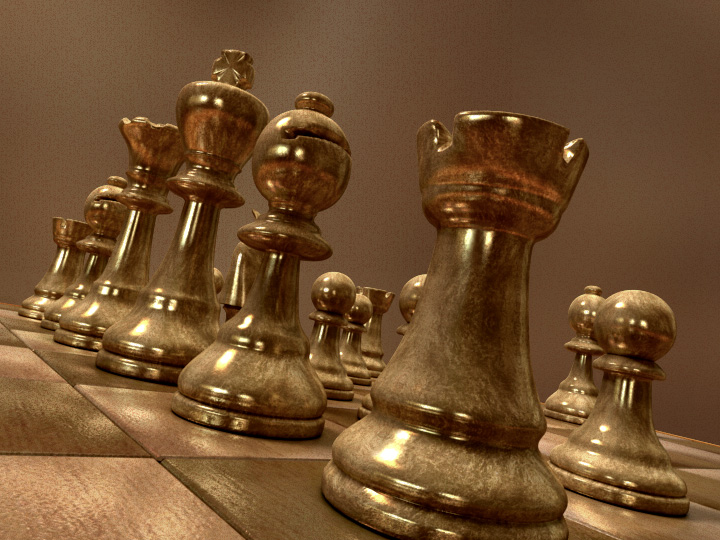
\includegraphics[width=.95\linewidth]{chess_rgb.jpg}
\end{subfigure}%
\begin{subfigure}{.5\textwidth}
  \centering
  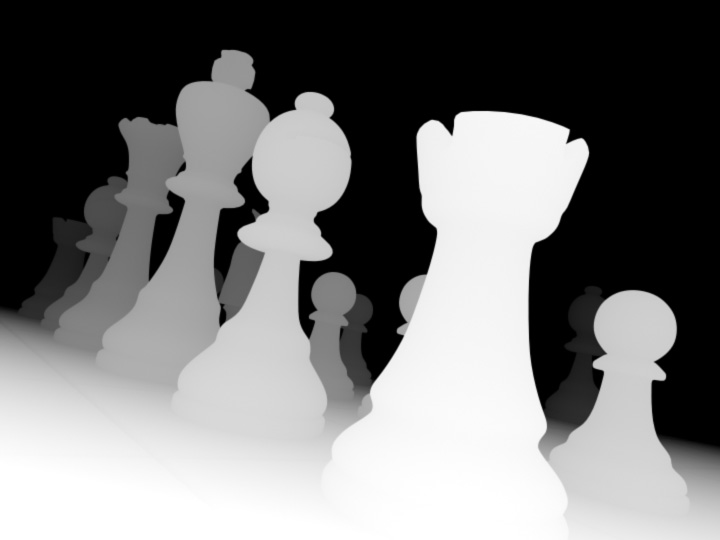
\includegraphics[width=.95\linewidth]{chess_d.jpg}
\end{subfigure}
\captionsetup{labelformat=empty}
\caption{Малюнак \cursection.\arabic{figure}: здымкі з RGB-D камеры}
\label{fig:rgbd-example}
\end{figure}

\renewcommand{\nextTitle}{2.2.3 Манакулярная RGB камера}
\addcontentsline{toc}{subsubsection}{\nextTitle}
\subsubsection*{\nextTitle}

Самымі распаўсюджанымі з'яўляюцца добра знаёмыя нам манакулярныя камеры - камеры, якія прысутнічаюць
у смартфонах і ўжываюцца ў быце.
Манакулярныя камеры, ў сваю чаргу, таксама бываюць розных тыпаў,
але на практыцы мы часцей за ўсё працуем з праектыўнымі (англ. ``projective'', ``pinhole'') камерамі.

Да таго ж гэта адзіны від камераў, з якімі ў рамках дадзенай работы вялася шчыльная праца,
для якіх рэалізаваныя алгарытмы і на якіх праводзіліся эксперыменты.

Праецыраванне трохмерных кропак у выпадку з манакулярнай камерай можа быць апісанае наступнай формулай:

\begin{equation}
  x = PX
\end{equation}

\vspace{4mm}

дзе $P$ - матрыца, якая здзяйсняе пераўтварэнне, $X, x$ - вектары, якія адпавядаюць
трохмернай і двухмернай кропцы адпаведна, запісаныя ў аднародных каардынатах.
У сваю чаргу матрыцу $P$ можна прадставіць як:

\begin{equation} \label{eq:transform-matrix}
  P = K[R|t]
\end{equation}

\vspace{4mm}

дзе $K$ - вектар унутраных параметраў камеры, $R$ - $3 \times 3$ матрыца павароту, $t$ - $3 \times 1$ вектар
зрушэння камеры ў прасторы ў сусветных каардынатах. Гэтыя параметры задаюць праектыўную
камеру, якая здзяйсняе праекцыю кропкі прасторы на матрыцу камеры. Унутраныя параметры могуць
задавацца разнастайным чынам, распаўсюджанымі прыкладамі выступаюць матрыцы:

\begin{equation}
  K = \begin{bmatrix}
    f & 0 & p_x \\[0.3em]
    0 & f & p_y \\[0.3em]
    0 & 0 & 1
  \end{bmatrix},
  \hspace{5mm}
  K = \begin{bmatrix}
    \alpha_x & 0 & p_x \\[0.3em]
    0 & \alpha_y & p_y \\[0.3em]
    0 & 0 & 1
  \end{bmatrix}
\end{equation}

\vspace{4mm}

дзе $f$ - фокусная адлегласць, $\alpha_x$, $\alpha_y$ - фокусная адлегласць уздоўж восяў
(для выпадкаў, калі не супадае), $p_x$, $p_y$ - зрушэнні цэнтру праекцыі адносна цэнтра матрыцы.
Іншымі параметрамі камеры могуць быць радыяльныя скажэнні $k_1, k_2$, якія ўзнікаюць з-за неідэальнасці
лінзаў у камерах.

\begin{figure}[h]
    \centering
    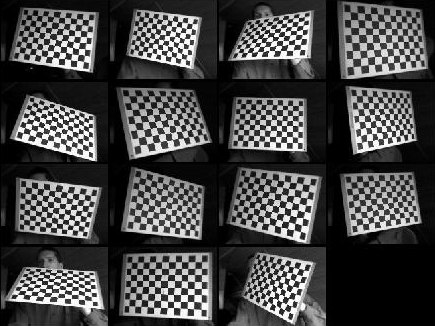
\includegraphics[width=0.8\textwidth]{calibration.jpg}
    \captionsetup{labelformat=empty}
    \caption{Малюнак \cursection.\arabic{figure}: працэс каліброўкі манакулярнай камеры}
    \label{fig:calibration}
\end{figure}

Унутраныя параметры камеры заўжды вядомыя загадзя альбо праз дакументацыю да прылады ад
вытворца, альбо праз каліброўку: каліброўка можа выяўляць хібы, дапушчаныя вытворцам.
Каліброўка дае добрыя значэнні ўнутраных параметраў
камеры, таму яны рэдка выкарыстоўваюцца ў якасці аптымізуемых параметраў.
Працэс каліброўкі, у выпадку патрэбы, не складана здзейсніць самастойна - існуе вялікая колькасць утылітаў
(напрыклад, у складзе OpenCV), якія дазваляюць гэта зрабіць, маючы ў наяўнасці толькі раздукаваную
дошку, якая нагадвае шахматную, памерамі 9x7 клетак (гэты параметр вар'юецца).
Працэс каліброўкі паказаны на малюнку \cursection.\ref{fig:calibration}.

У сваю чаргу, матрыца $R$ і вектар $t$ ва ўраўненні \ref{eq:transform-matrix} з'яўляюцца
\textit{знешнімі параметрамі камеры} і вызначаюцца пазіцыяй камеры ў прасторы.

Варта зазначыць, што адной з найбольшых перавагаў і, адначасова, адной з найбольшых
перашкодаў у працы ў манакулярнымі камерамі з'яўляецца неадназначнасць працы з масштабам.
Праблема ў тым, што масштаб не можа быць высветлены праз перасоўванні ў прасторы і
змяненні ў вуглах агляду, што з'яўляецца крыніцай мноства памылак. Разам з тым,
перавага неадназначнасці масштабу ва ўніверсальнасці: алгарытм будзе працаваць
з аднолькавымі вынікамі як у маленькіх закрытых памяшканнях, так і на вялікіх
адкрытых прасторах. З гэтым аспектам (немачыгмасць высвятлення рэальных памераў аб'ектаў)
мы яшчэ сутыкнемся пры абмеркаванні SLAM-алгарытмаў - некаторыя з іх, такія як
CNN-SLAM (\cite{DBLP:journals/corr/TatenoTLN17}), прапаноўваюць шляхі вырашэння гэтай праблемы.

\subsubsection*{Заданне матрыцы павароту праз кватэрніоны}

\vspace{5mm}

Альтэрнатывай апісанай вышэй матрыцы павароту памера $3 \times 3$
можа быць апісанне павароту з дапамогай кватэрніонаў.

{\bf Кватэрніоны} - сістэма гіперкамплексных лікаў,
якія ўтвараюць вектарную прастору размернасцю 4 над полем рэчаісных лікаў.

Кватэрніон можа быць прадстаўлены як фармальная сума
$q(a, b, c, d) = a + bi + cj + dk$, дзе $a, b, c, d \in\mathbb{R}$, $i, j, k$ -
уяўныя адзінкі, такія, што $i^2 = j^2 = k^2 = ijk = -1$.

Кватэрніон часта запісываецца як пара $(a, \vec{u})$, дзе $a \in\mathbb{R}$,
$\vec{u} = (b, c, d) \in\mathbb{R}^3$ - вектар у трохмернай прасторы,
што дае нагоду задумацца аб прымяненні кватэрніонаў для заданняў паваротаў у трохмернай прасторы.

Негледзячы на тое, што агулам кватэрніоны не знайшлі шырокага прымянення,
іх выкарыстанне часта апраўданае ў некаторых галінах матэматыкі ды інфарматыкі,
такіх як камп'ютарная графіка, навігацыя альбо праграмаванне гульняў.
Кватэрніоны мінімальнай колькасцю скалярных параметраў задаюць паварот,
пры гэтым яны пазбаўленыя выраджанасці, якая сустракаецца пра заданні паварота
пры дапамозе толькі трох параметраў (напрыклад - вугламі Эйлера).

Калі маем кватэрніон $q = (w, x, y, z)$, тады матрыца павароту можа быць запісаная праз кватэрніон як:
\begin{equation} \label{eq:quaternion-to-rotation}
    R = \left( \begin{array}{ccc}
    1 - 2y^2 - 2z^2 & 2xy - 2zw & 2xz + 2yw \\
    2xy + 2zw & 1 - 2x^2 - 2z^2 & 2yz - 2xw \\
    2xz - 2yw & 2yz + 2xw & 1 - 2x^2 - 2y^2 \end{array} \right)
\end{equation}

У практычнай рэалізацыі з главы 4 кватэрніоны выкарыстоўваюцца пры перадачы знешніх
параметраў камер паміж кампанентамі сістэмы,
схематычна прадстаўленай на малюнку 4.\ref{fig:architecture}.

\renewcommand{\nextTitle}{2.3 Ключавыя кропкі, дэскрыптары, спосабы іх апісання}
\addcontentsline{toc}{subsection}{\nextTitle}
\subsection*{\nextTitle}

\vspace{5mm}

Тут і далей мы будзем казаць пра ``ключавыя кропкі'' (англ. \textit{keypoints})
альбо ``асаблівасці'' (англ. \textit{features}), хаця ў тэрмінах таго ці іншага дэтэктара
ключавой кропкай можа называцца любая адзінка інфармацыі: кропка, акружнасць, лінія, вектар і інш.

Дэтэктарам (англ. \textit{detector}) будзем называць алгарытм, які знаходзіць на выяве ключавыя кропкі.

Знойдзеная ключавая кропка пасля звычайна апісваецца ў нейкай вызначанай кароткай форме. Такое апісанне ключавой кропкі
называецца дэскрыптарам (англ. \textit{descriptor}). Часцей за ўсё сустракаюцца дэскрыптары ў выглядзе рэчаісных
вектароў альбо бінарных радкоў. Дэскрыптары дапамагаюць хутка знаходзіць адпаведныя адна адной ключавыя кропкі на
розных выявах. Знайсці адлегласць паміж двумя дэскрыптарамі і, такім чынам, вызначыць іхняе падабенства, з'яўляецца
асноўнай аперацыяй пры пошуку адпаведнасцяў паміж дзвюма выявамі, таму да надзейнасці і хуткасці падліку функцыі адлегласці
прад'яўляюцца асаблівыя патрабаванні. На практыцы адлегласць часцей за ўсё падлічваецца праз Эўклідаву адлегласць L2 (для
рэчаісных вектароў) альбо праз адлегласць Хэмінга (для бінарных радкоў).

\begin{figure}[h]
    \centering
    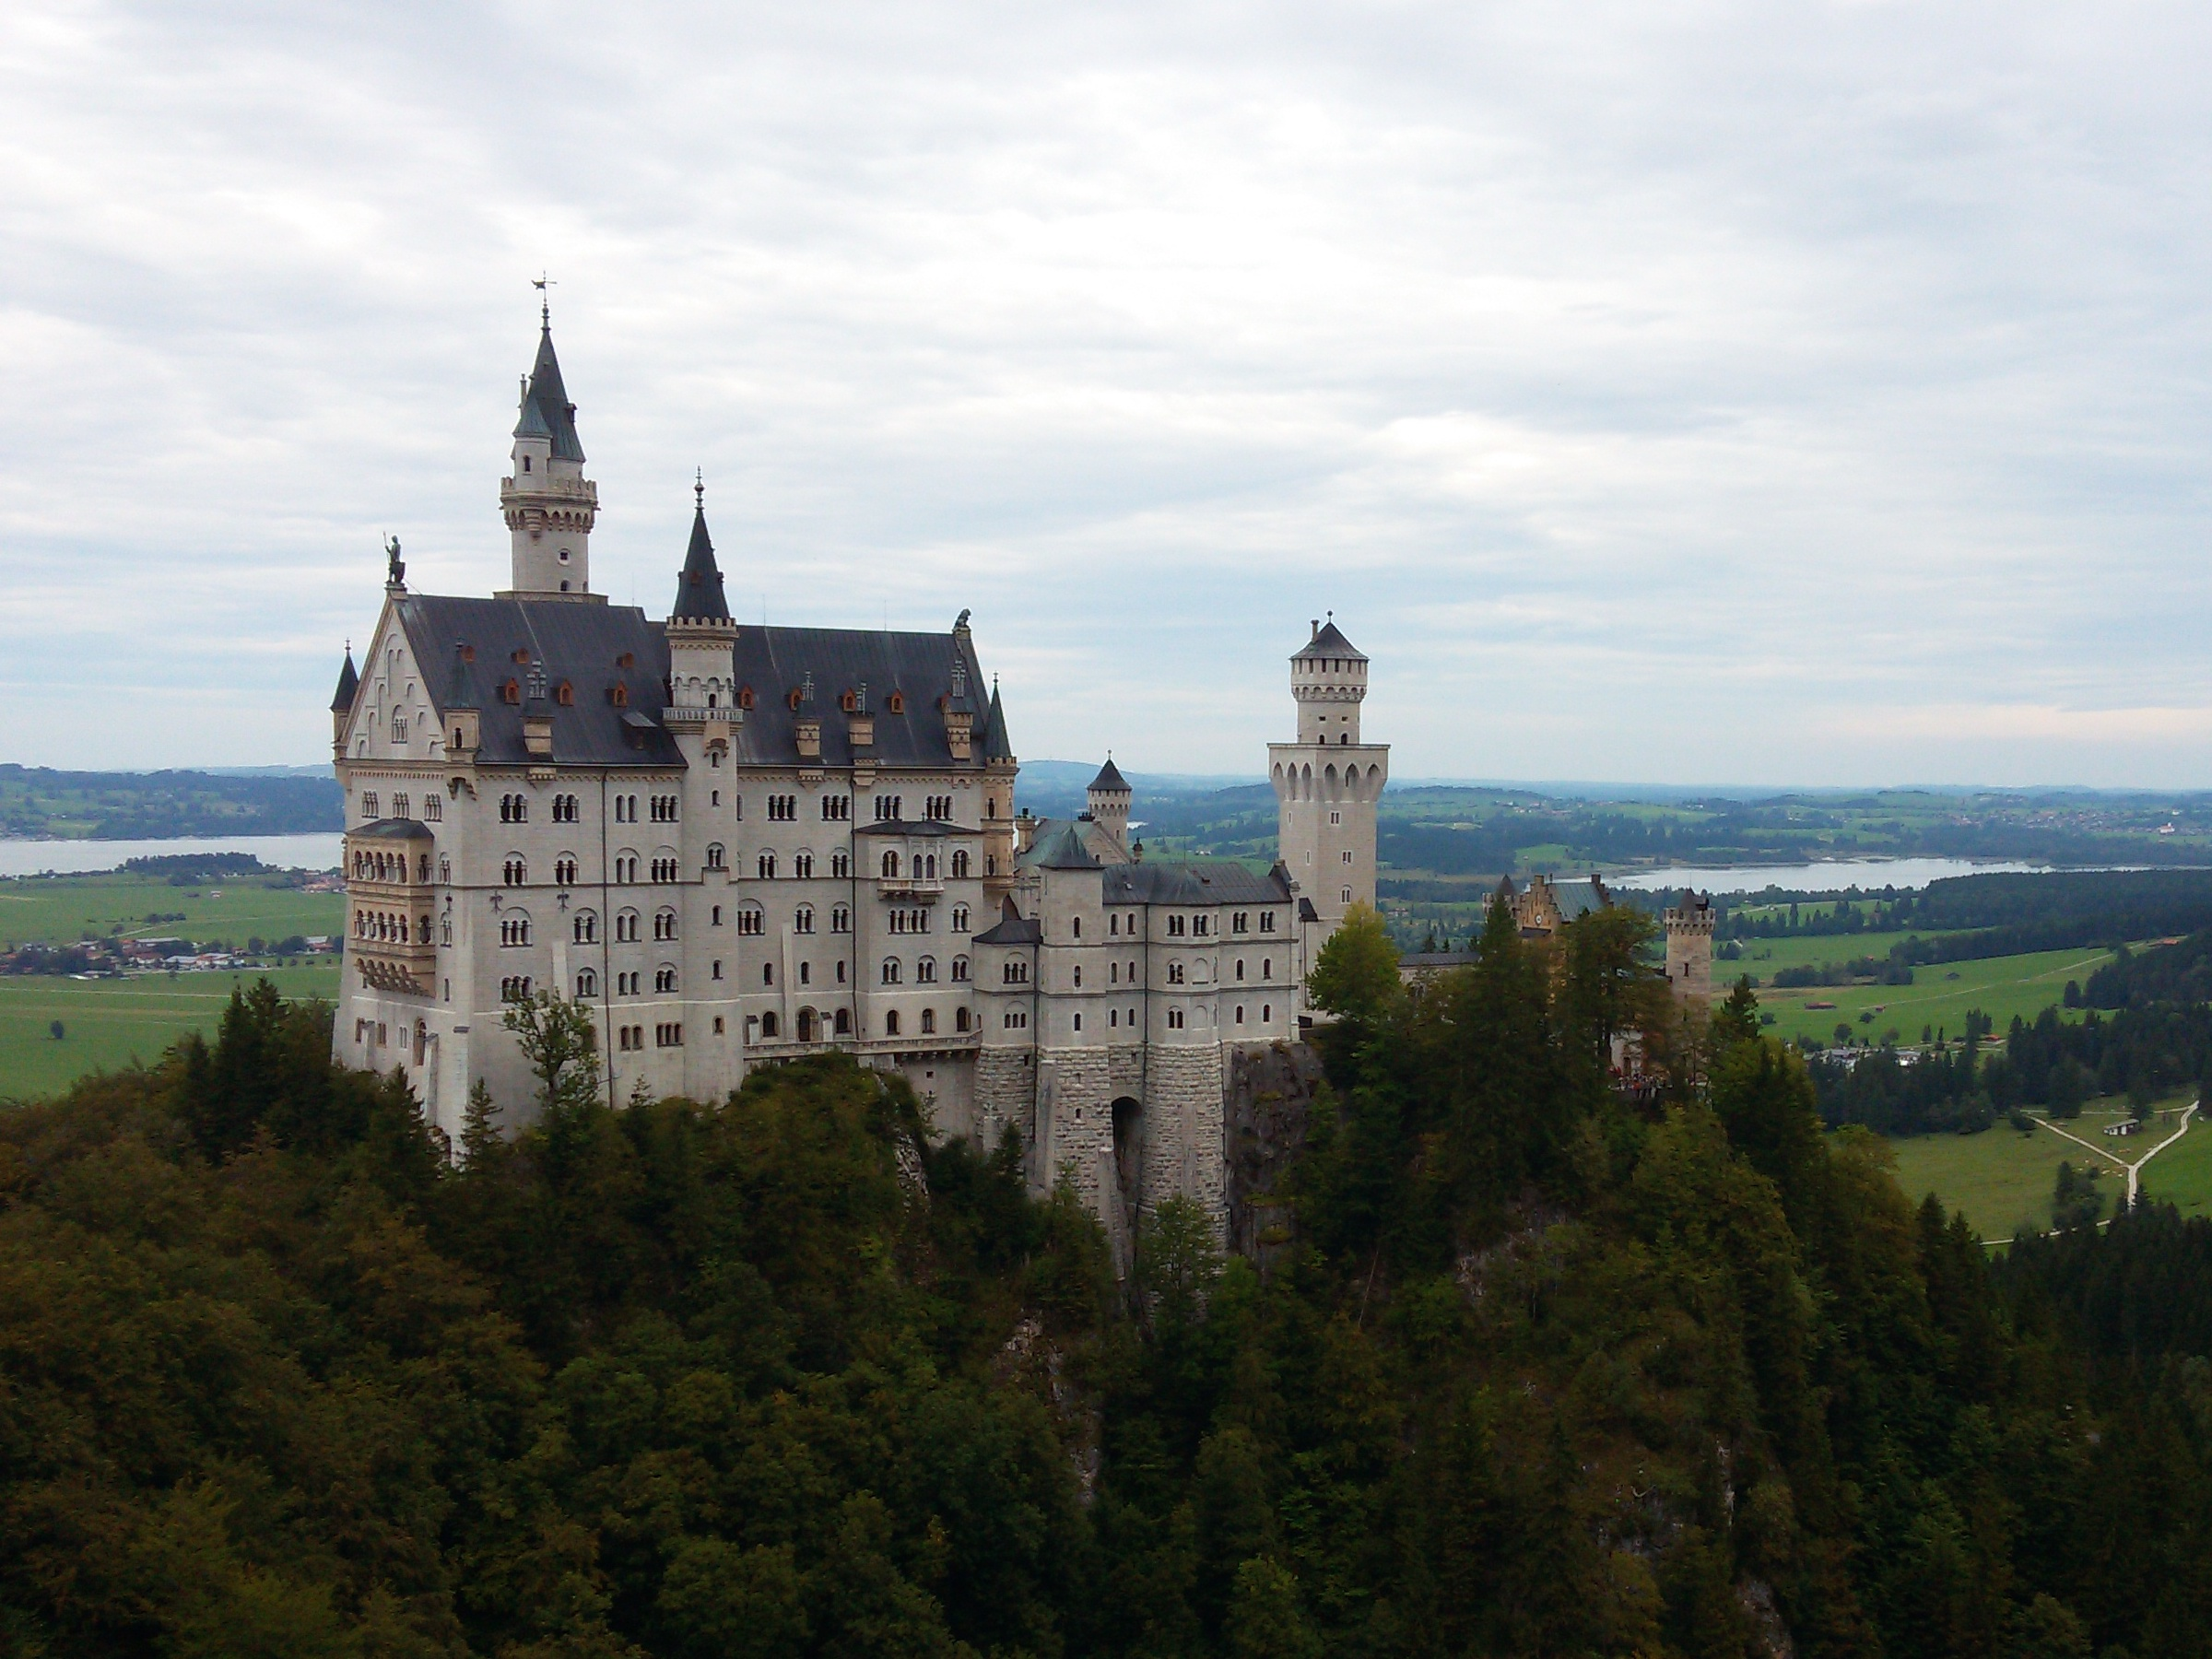
\includegraphics[width=0.8\textwidth]{castle0.jpg}
    \captionsetup{labelformat=empty}
    \caption{Малюнак \cursection.\arabic{figure}: зыходная выява}
    \label{fig:sift0}
\end{figure}

\begin{figure}[t]
    \centering
    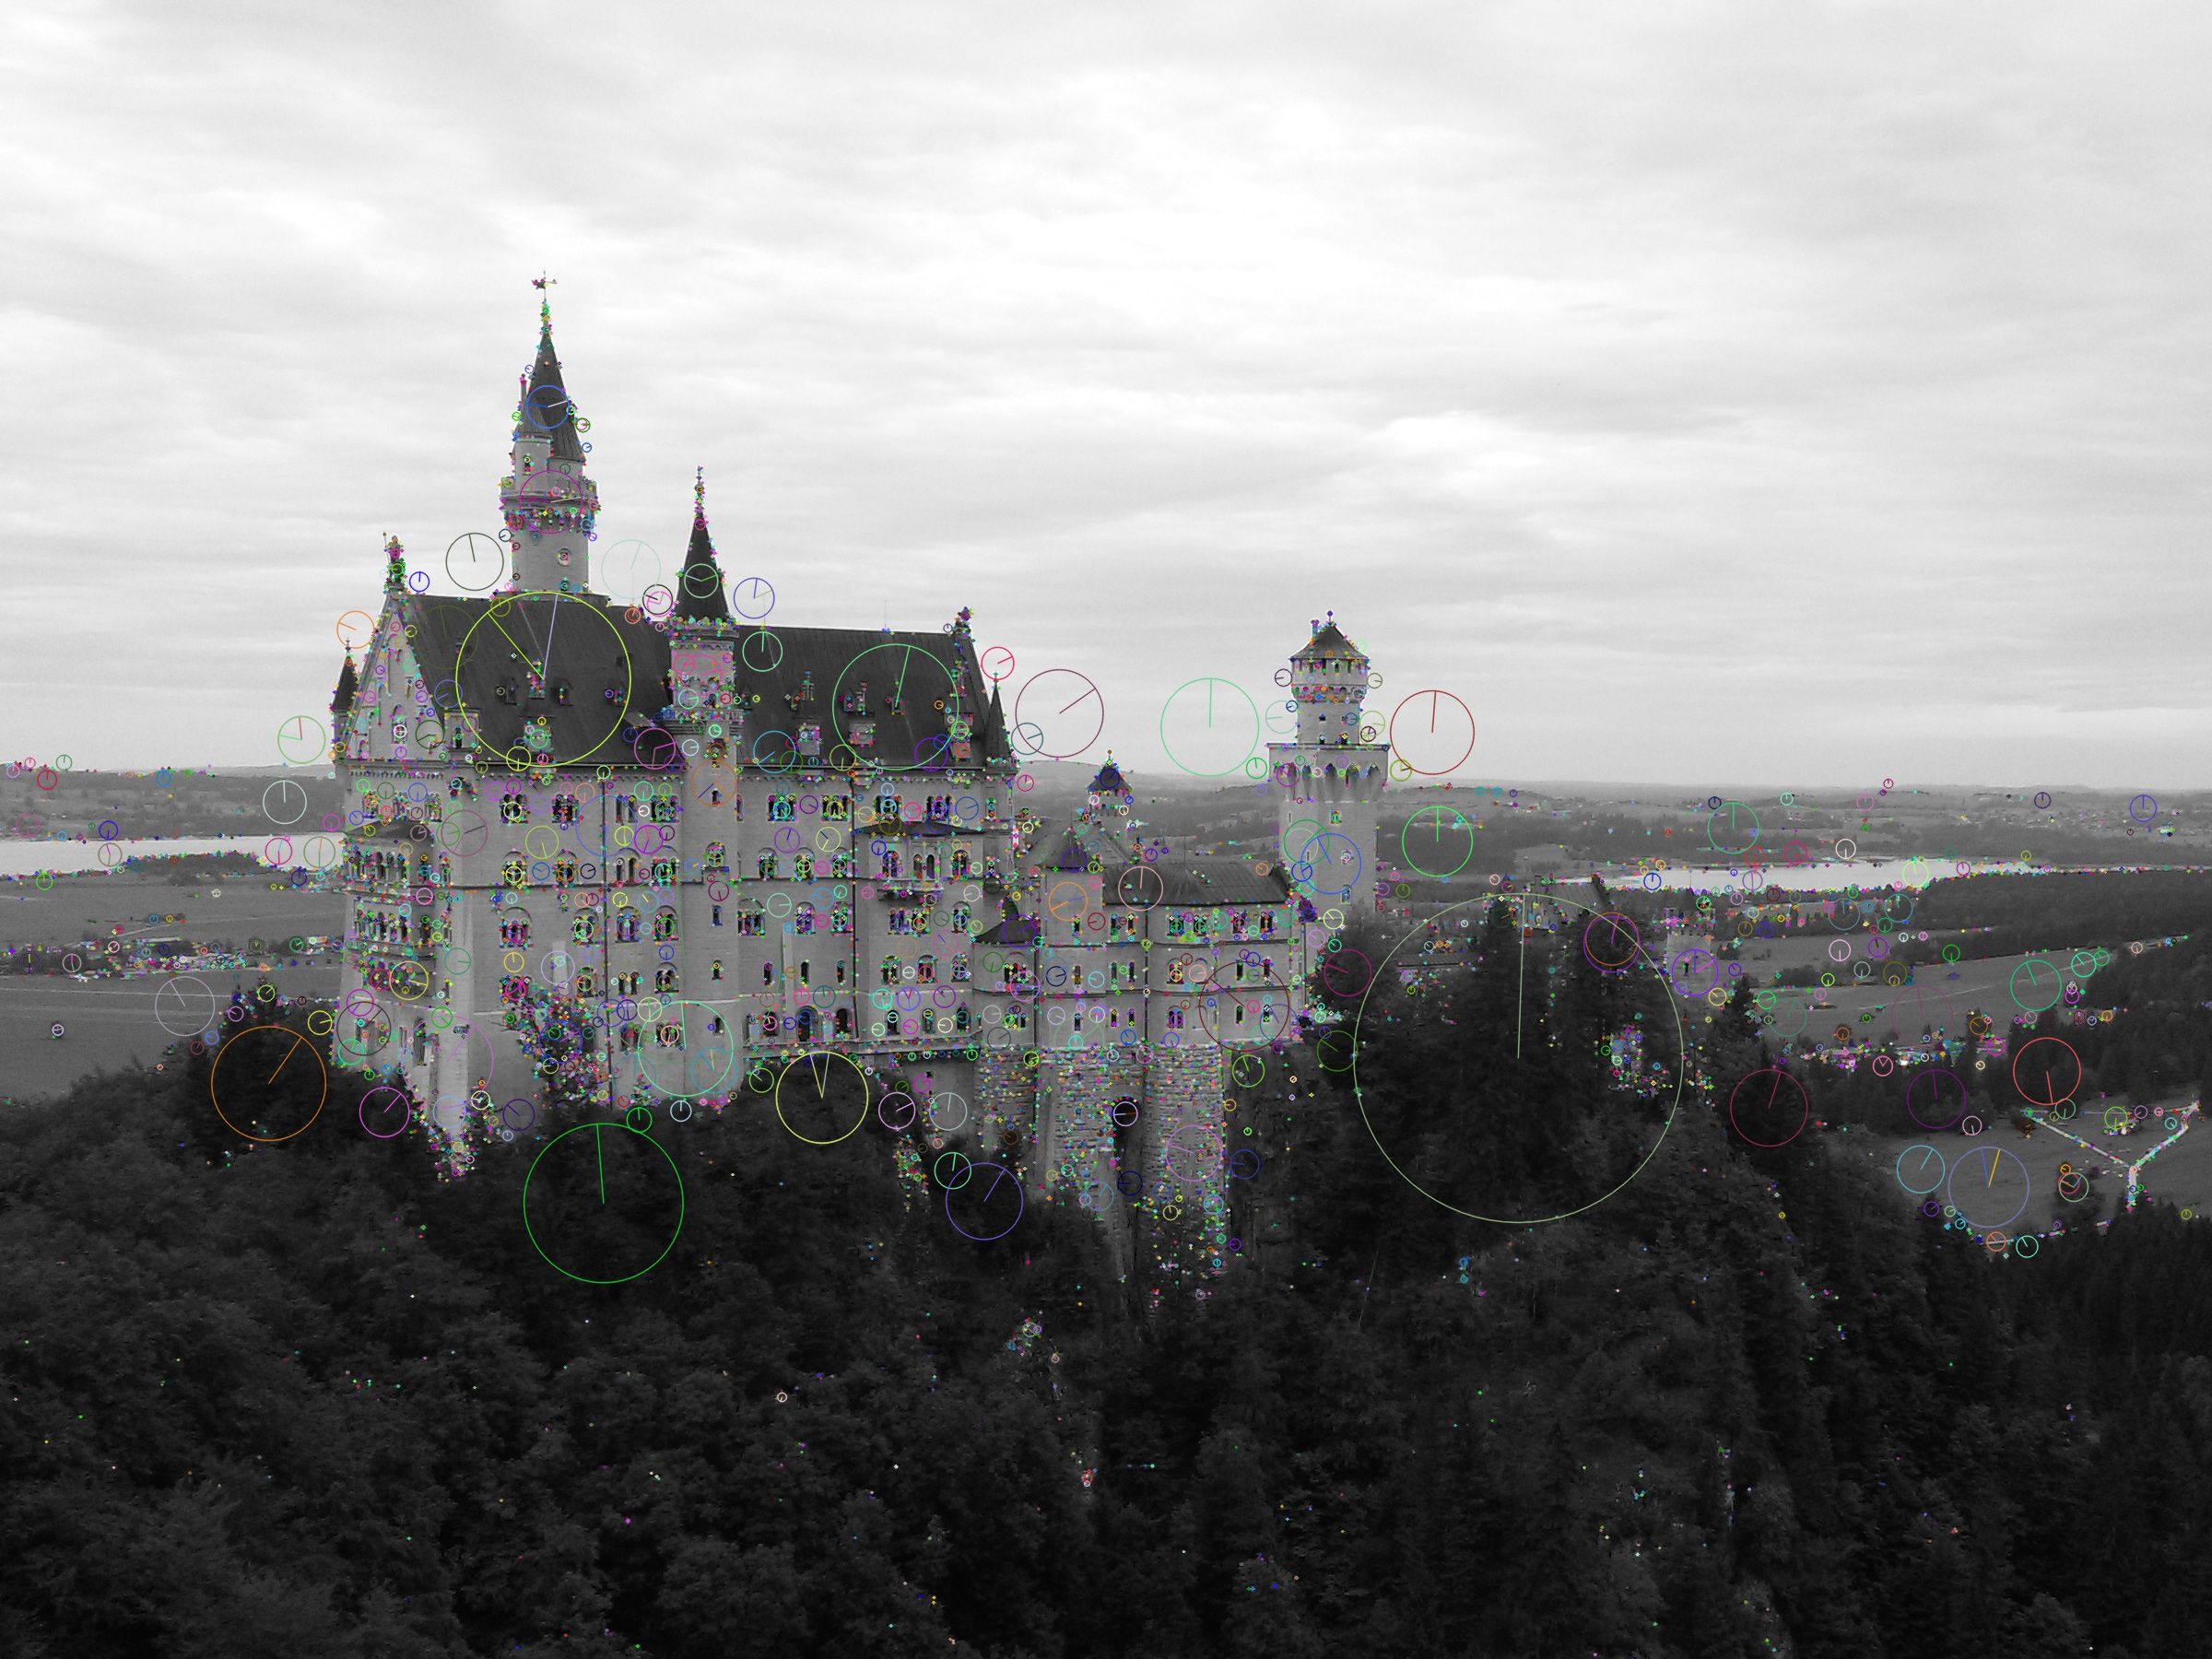
\includegraphics[width=0.8\textwidth]{castle0_sift.jpg}
    \captionsetup{labelformat=empty}
    \caption{Малюнак \cursection.\arabic{figure}: выява з нанесенымі ключавымі кропкамі (SIFT)}
    \label{fig:sift1}
\end{figure}

\vspace{5mm}

Ніжэй прыведзенае кароткае апісанне найбольш распаўсюджаных дэтэктараў ключавых кропак і спосабаў іх апісання.

\renewcommand{\nextTitle}{2.3.1 Апісанне некаторых распаўсюджаных дэтэктараў і дэскрыптараў}
\addcontentsline{toc}{subsubsection}{\nextTitle}
\subsubsection*{\nextTitle}

\vspace{5mm}

Дэтэктар \textbf{FAST} (\textit{Features from Accelerated Segment Test}) \cite{fast-paper}.
Як вынікае з назвы, асноўнай перавагай дэтэктара
з'яўляецца ягоная хуткасць, што асабліва важна ў выпадку, калі дадзеныя паступаюць
і патрабуюць апрацоўкі ў рэжыме рэальнага часу і абмежаваных рэсурсаў.
Найлепшым прыкладам будуць SLAM-прыкладанні (\textit{Simultaneous Localization and Mapping}),
у якіх у рэжыме рэальнага часу адбываецца ацэнка месцазнаходжання і пошук яго на мапе;
SLAM-прыкладанні часта знаходзяць прымяненне на мабільных прыладах, у тым ліку на БПЛА.

FAST з'яўляецца алгарытмам ``пошуку вуглоў'' (англ. \textit{corner detector}):
кропка з'яўляецца ключавой, калі ў маленькіх ваколіцах пікселя алгарытму атрымліваецца
распазнаць адпаведны шаблон, іншымі словамі ``вугал''.
Дадатковая аптымізацыя адбываецца з дапамогай метадаў машыннага навучання.

Даследаванні паказваюць, што ён у некалькі разоў хутчэйшы за іншыя існуючыя алгарытмы пошука ключавых кропак на аснове
вылучэння вуглоў, але, у сваю чаргу, ён недастаткова ўстойлівы да моцна зашумленых выяваў.

\vspace{5mm}

Дэскрыптар і дэтэктар \textbf{SIFT} \cite{sift-paper} быў прадстаўлены ў 2004 годзе і
па стане на сёння з'яўляецца адным з найбольш распаўсюджаных.
Важнымі характарыстыкамі алгарытмамі з'яўляецца ўстойлівасць да масштабавання і
змянення арыентацыі выявы, яе афінных пераўтварэнняў
і зашумленых варыянтаў. Яскрава выраджаная характэрнасць ключавых кропак дазваляе
паспяхова шукаць адпаведнасці паміж
рознымі выявамі. У \cite{sift-paper}, апроч апісання спосаба вымання ключавых кропак
і фармата дэскрыптара, апісваюцца тэхнікі для
эфектыўнага пошука адпаведнасцяў паміж выявамі з SIFT дэскрыптарамі,
а таксама алгарытмы эфектыўнага распазнавання патэрнаў.
Такая завершанасць даследавання алгарытма дае яму вялікую перавагу перад
іншымі і моцна паспрыяла ягонаму распаўсюду.
SIFT дэскрыптарам з'яўляецца рэчаісны вектар размернасці 128.

На малюнку \cursection.\ref{fig:sift1} можна бачыць візуалізацыю знойдзеных
алгарытмам SIFT ключавых кропак па пачатковым малюнку \cursection.\ref{fig:sift0}.

Дэскрыптар і дэтэктар \textbf{SURF} \cite{surf-paper} быў упершыню апублікаваны ў 2006 годзе
і пачаткова ідэя стварэння заключалася ў стварэнне ``больш хуткага'' SIFT-а.
Ён таксама з'яўляецца ўстойлівым да змены масштаба і паварота, можа быць паспяхова прыменены
для размытых выяваў; разам з тым, выкарыстанне SURF-а абмежаванае,
калі мы маем справу са зменамі ў вугле назірання. Дэскрыптар SURF
можа быць як размернасці 64, так і 128 (як SIFT).

Звернем увагу на тое, што і SIFT і SURF з'яўляюцца запатэнтаванымі алгарытмамі і,
негледзячы на вялікую колькасць рэалізацыяў з адкрытым
зыходным кодам, іх выкарыстанне ў камерцыйных прадуктах абмежаванае.
У сваю чаргу, алгарытм ORB прапрыетарным не з'яўляецца.

\vspace{5mm}

Дэскрыптар і дэтэктар \textbf{ORB} (\textit{Oriented FAST and Rotated BRIEF}) \cite{orb-paper}
з'яўляецца своеасаблівай камбінацыяй ключавых кропак FAST і дэскрыптара BRIEF.
Мэтай стварэння ORB было пераўзысці SIFT у хуткасці (нават ахвяруючы надзейнасцю і дакладнасцю)
у сувязі з распаўсюдам мабільных маламагутных прыладаў. Дэскрыптары маюць выгляд бінарных радкоў.
Адпаведнасці паміж ORB дэскрыптарамі эфектыўна могуць быць знойдзеныя з дапамогай LSH (Locality-sensitive hashing).

\vspace{5mm}

Дэскрыптар \textbf{BRIEF} (\textit{Binary Robust Independent Elementary Features}) \cite{brief-paper}
стаў адным з першых дэскрыптараў, якія апісываюць ключавыя кропкі
з дапамогай бінарных радкоў (SIFT альбо SURF, напрыклад, выкарыстоўваюць вектары
з рэчаіснымі лікамі якія, у большасці выпадкаў, пасля ўсё адно ў мэтах эфектыўнасці
фарматуюцца ў бінарныя радкі, што дазваляе выкарыстоўваць эфектыўную адлегласць Хэмінга).

\vspace{5mm}

Дэскрыптар і дэтэктар \textbf{BRISK} (\textit{Binary Robust Invariant Scalable Keypoints})
\cite{brisk-paper} ствараўся як альтэрнатыва вышэйзгаданым SIFT i SURF,
хуткасць працы якога дасягаецца праз выкарыстанне новага, заснаванага на FAST, дэтэктара
ў камбінацыі з бінарным дэскрыптарам.

\vspace{5mm}

Звернем увагу на тое, што некаторыя алгарытмы спалучаюць у сабе адразу як пошук ключавых кропак, так і падлік іх
дэскрыптараў. У агульным выпадку гэты працэс можа быць яўна падзелены: на мностве ключавых кропак атрыманых любым з дэтэктараў
можа быць запушчаны алгарытм, які для кожнай кропцы паставіць у адпаведнасць дэскрыптар вызначанага фармата.
На практыцы, некаторыя пары дэтэктара і дэскрыптара спалучаюцца добра і заўжды выкарыстоўваюцца разам, некаторыя сумяшчаюцца
вельмі кепска. Большасць алгарытмаў, якія знайшлі шырокае прымяненне, апісываюць адразу спосаб дэтэкцыі і апісання і ўтвараюць
такім чынам закрытую сістэму, раздзяленне якой не прыводзіць да добрых вынікаў.

Даследванне спалучальнасці разам разнастайных дэтэктараў і дэскрыптараў праводзіліся мной у рамках
курсавой працы.

\renewcommand{\nextTitle}{2.4 Спалучэнне простых метадаў і метадаў, заснаваных на ключавых кропках}
\addcontentsline{toc}{subsection}{\nextTitle}
\subsection*{\nextTitle}

\vspace{5mm}

Вядомыя эфектыўныя алгарытмы, якія спалучаюць у сабе простыя метады і метады,
заснаваныя на выманні асаблівасцяў. Найбольшы распаўсюд такія алгарытмы знайшлі
ў задачах апрацоўкі плыні дадзеных (відэаплыня, апрацоўка дадзеных у рэальным часе з БПЛА),
калі алгарытм будуе мапу мясцовасці і шукае сваё месцазнаходжанне ў рэальным часе.

Напрыклад, у \cite{Forster2014ICRA} яўны пошук асаблівасцяў выклікаецца толькі калі
новы кадр запускае ініцыялізацыю новых трохмерных кропак у прасторы, іначай
выкарыстоўваюцца простыя метады якія, у сваю чаргу, няяўна даюць адпаведнасці паміж кропкамі,
пазначанымі раней у якасці асаблівых.

\renewcommand{\nextTitle}{2.5 Пошук адпаведнасцяў паміж ключавымі кропкамі}
\addcontentsline{toc}{subsection}{\nextTitle}
\subsection*{\nextTitle}

Пошук асаблівых кропак і падлік адпаведных дэскрыптараў з'яўляецца, вядома ж,
толькі падрыхтоўчым этапам да этапа параўнання дэскрыптараў з
дзвюх выяваў і пошуку найлепшых параў (працэс матчынга, англ. \textit{feature matching}).
Не існуе ўніверсальнага спосаба, які даваў бы найлепшыя
вынікі на любым тыпе асаблівых кропак і іх дэскрыптараў: для кожнага набора
дэскрыптараў існуе найбольш эфектыўны спосаб пошуку адпаведнасцяў.
Таксама, выбар алгарытма залежыць ад пастаўленых намі задачаў і расстаўленых прыарытэтаў:
ці нам найважнейшая хуткасць ці дакладнасць, ці дастаткова нам толькі $n$ найлепшых супадзенняў
ці мы хочам атрымаць усе знойдзеныя. Важным пытаннем з'яўляецца вызначэнне парога,
калі знойдзеная пара дэскрыптараў з'яўляецца заведама хібнай.

\begin{figure}[h]
    \centering
    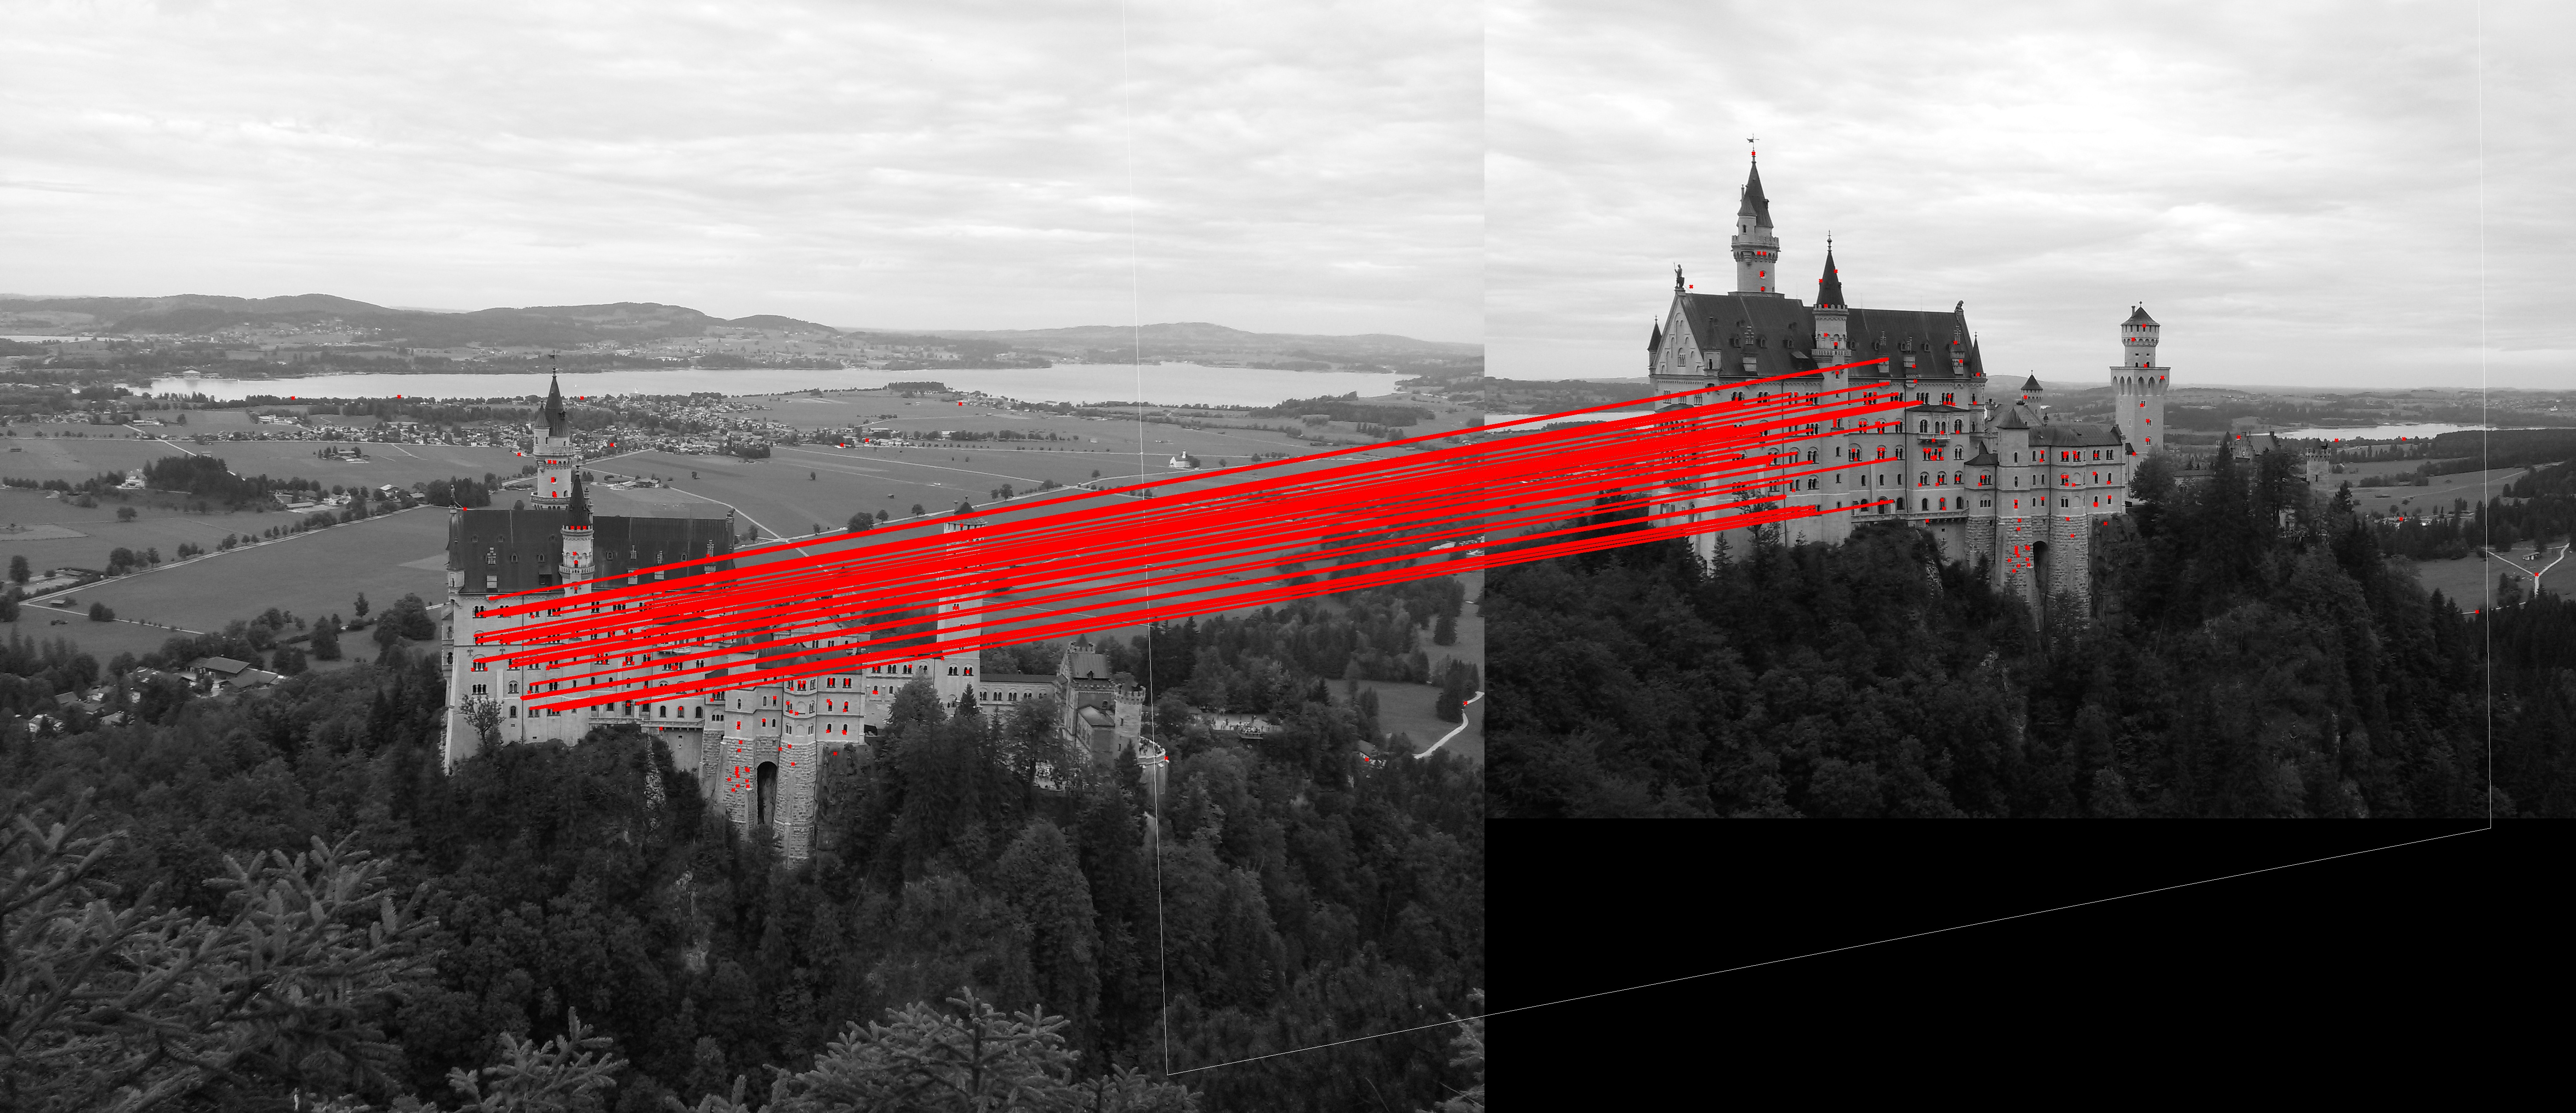
\includegraphics[width=1.0\textwidth]{castle_matches.jpg}
    \captionsetup{labelformat=empty}
    \caption{Малюнак \cursection.\arabic{figure}: вынік пошуку адпаведнасцяў паміж ключавымі кропкамі}
    \label{fig:matches}
\end{figure}

Самым простым спосабам знайсці адпаведнасці паміж дэскрыптарамі з дзвюх розных выяваў
з'яўляецца просты пералік усіх магчымых параў, падлік нормы (L2, Хэмінга, альбо любой іншай)
і сартыроўка ўсіх параў па ўзрастанні значэнняў адлегласцяў (гэтак званы Brute-Force Matcher).
Такі спосаб з'яўляецца простым у рэалізацыі, беспамылковым, але вельмі марудным.
Практычнае прымяненне ва ўмовах апрацоўкі плыняў дадзеных альбо
пры пост-апрацоўцы вялікіх набораў дадзеных часта немагчымае.

Для выпадкаў, калі дакладнасцю можна ахвяраваць на карысць хуткасці (напрыклад, у працы з БПЛА хуткасць апрацоўкі
грае першасную ролю), былі вынайдзеныя і іншыя алгарытмы пошуку адпаведнасцяў.

Метады, пра якія ідзе гаворка, маюць агульную назву \textit{метадаў набліжанага пошуку бліжэйшых суседзяў}
(англ. \textit{Approximate Nearest Neighbors}). Падлічаныя намі дэскрыптары з'яўляюцца звычайным мноствам вектароў,
на якім зададзеныя суадносіны адлегласці. У практычнай частцы такія метады будуць выкарыстоўвацца.
Для дэскрыптараў з рэчаіснымі вектарамі (SIFT, SURF) гэта будзе метад заснаваны на k-мерных дрэвах
(англ. \textit{k-dimensional trees}), для бінарных дэскрыптараў - Locality-sensitive Hashing (LSH) - імавернасны
метад паніжэння размернасці дадзеных.

На малюнку \cursection.\ref{fig:matches} можна бачыць нанесеныя простыя лініі, якія злучаюць кропкі,
адпаведныя адной і той жа кропцы прасторы.
Дэскрыптары былі падлічаныя алгарытмам SIFT.

\renewcommand{\nextTitle}{2.6 Фармальная пастаноўка задачы рэканструкцыі}
\addcontentsline{toc}{subsection}{\nextTitle}
\subsection*{\nextTitle}

\vspace{5mm}

Задача аднаўлення трохмерных каардынатаў кропак па наборы выяваў,
зробленых з розных ракурсаў і пазіцыяў, атрымала агульную назву
задачы пучковай аптымізацыі (англ. {\bf bundle adjustment}).
Задача заключаецца ў мінімізацыі памылкі функцыянала, які задае суадносіны паміж
мноствам кропак прасторы і праекцыямі гэтых кропак. Строга гэта можа быць запісана як:

\begin{equation} \label{eq:bundle-adjustment}
    \min_{a_j, b_i} \sum_{i=1}^{n} \sum_{j=1}^{m} v_{ij}d(Q(a_j, b_i), x_{ij})^2
\end{equation}

\vspace{4mm}

дзе:\\
$n$ - колькасць кропак у трохмернай прасторы, якія бачныя хаця б на адным фотаздымку,\\
$m$ - колькасць выяваў (колькасць камер),\\
$x_{ij}$ - праекцыя кропкі $i$ на выяву $j$,\\
$v_{ij}$ - дваічная зменная, якая вызначае, ці бачная кропка $i$ на выяве $j$,\\
$a_{j}$ - вектар параметраў камеры $j$,\\
$b_{i}$ - набліжэнне для кропкі $i$ прасторы,\\
$Q(a_j, b_i)$ - функцыя пошуку праекцыі кропкі $i$ на выяву $j$,\\
$d(x, y)$ - Эўклідава адлегласць паміж кропкамі $x$ i $y$.

\vspace{4mm}

Мінімізаваўшы памылку функцыянала, мы знойдзем найлепшае магчымае набліжэнне для
параметраў камераў $a_{j}$ і кропак трохмернай прасторы $b_{i}$,
што дасць нам магчымасць зрабіць візуалізацыю мадэлі, што і з'яўляецца нашай мэтай.

Дадзеная задача можа рашацца як агульнымі падыходамі да мінімізацыі функцыяналу,
так і спецыяльна распрацаванымі алгарытмамі, якія ўлічваюць разрэджаную структуру матрыцы,
якая апісвае функцыянал, такім чынам эфектыўна рашаючы задачу пучковай аптымізацыі.
Алгарытмам, які атрымаў найбольшы распаўсюд пры практычнай рэалізацыі,
з'яўляецца алгарытм Левенберга-Марквардта (англ. \textit{Levenberg–Marquardt algorithm, LMA}).
Гэта ітэратыўны алгарытм рашэння задачы мінімізацыі нелінейнага функцыянала спосабам
найменшых квадратаў (англ. \textit{non-linear least squares problem}).

\newpage
